\documentclass{beamer}
\usepackage[utf8]{inputenc}

\usetheme{Madrid}
\usecolortheme{default}
\usepackage{amsmath,amssymb,amsfonts,amsthm}
\usepackage{txfonts}
\usepackage{tkz-euclide}
\usepackage{listings}
\usepackage{adjustbox}
\usepackage{array}
\usepackage{tabularx}
\usepackage{gvv}
\usepackage{lmodern}
\usepackage{circuitikz}
\usepackage{tikz}
\usepackage{graphicx}
\usepackage{caption}
\captionsetup{labelformat=empty}  % removes "Figure:"


\setbeamertemplate{page number in head/foot}[totalframenumber]

\usepackage{tcolorbox}
\tcbuselibrary{minted,breakable,xparse,skins}



\definecolor{bg}{gray}{0.95}
\DeclareTCBListing{mintedbox}{O{}m!O{}}{%
	breakable=true,
	listing engine=minted,
	listing only,
	minted language=#2,
	minted style=default,
	minted options={%
		linenos,
		gobble=0,
		breaklines=true,
		breakafter=,,
		fontsize=\small,
		numbersep=8pt,
		#1},
	boxsep=0pt,
	left skip=0pt,
	right skip=0pt,
	left=25pt,
	right=0pt,
	top=3pt,
	bottom=3pt,
	arc=5pt,
	leftrule=0pt,
	rightrule=0pt,
	bottomrule=2pt,
	toprule=2pt,
	colback=bg,
	colframe=orange!70,
	enhanced,
	overlay={%
		\begin{tcbclipinterior}
			\fill[orange!20!white] (frame.south west) rectangle ([xshift=20pt]frame.north west);
	\end{tcbclipinterior}},
	#3,
}
\lstset{
	language=C,
	basicstyle=\ttfamily\small,
	keywordstyle=\color{blue},
	stringstyle=\color{orange},
	commentstyle=\color{green!60!black},
	numbers=left,
	numberstyle=\tiny\color{gray},
	breaklines=true,
	showstringspaces=false,
}
\begin{document}

\title 
{4.3.35}
\date{October 1,2025}

\author 
{Navya Priya - EE25BTECH11045}
\graphicspath{./figs}

\frame{\titlepage}
\begin{frame}{Question}
    Find the intercepts made by the plane $2\text{x} - 3\text{y} + 5\text{z} + 4 = 0$ on the co-ordinate axis 
\end{frame}

\begin{frame}{Theoretical Solution}
   The above equation of plane can be written as
\begin{align*}
    \vec{n}^\top \vec{x}\,=\,\text{c}
\end{align*}
where 
\begin{align}
    \vec{n}=\myvec{2\\-3\\5}\\
    \text{c}=-4
\end{align}
\end{frame}

\begin{frame}{X-intercept}
Let the x-intercept of the given plane be of the form $\myvec{a\\0\\0}$. Substituting this in the above equation gives
\begin{align}
   \myvec{2\\-3\\5}^\top \myvec{a\\0\\0}\,&=\,-4\\
    \text{a}&=\,-2
\end{align}
\begin{align*}
    \therefore \,\text{The}\, x-\text{intercept \,is\,} \myvec{-2\\0\\0}
\end{align*}
\end{frame}

\begin{frame}{Y-intercept}
Let the y-intercept of the given plane be of the form $\myvec{0\\b\\0}$. Substituting this in the above equation gives
\begin{align}
   \myvec{2\\-3\\5}^\top \myvec{0\\b\\0}\,&=\,-4\\
    \text{b}&=\,\frac{4}{3}
\end{align}
 \begin{align*}
    \therefore \,\text{The}\, y-\text{intercept \,is\,} \myvec{0\\\frac{4}{3}\\0}
\end{align*} 
\end{frame}

\begin{frame}{Z-intercept}
 Let the z-intercept of the given plane be of the form $\myvec{0\\0\\c}$. Substituting this in the above equation gives
\begin{align}
   \myvec{2\\-3\\5}^\top \myvec{0\\0\\c}\,&=\,-4\\
    \text{c}&=\,\frac{-4}{5}
\end{align}
\begin{align*}
    \therefore \,\text{The}\, z-\text{intercept \,is\,} \myvec{0\\0\\\frac{-4}{5}}
\end{align*}
\end{frame}

\begin{frame}[fragile]{C code}
\begin{lstlisting}
#include <stdio.h>

void find_intercepts(double *x_int, double *y_int, double *z_int,double a,double b,double c,double d) {
    // Plane equation: ax + by + cz = d
    // X-intercept -> y=0, z=0 -> ax=d 
    *x_int = d.0 / a.0;

    // Y-intercept -> x=0, z=0 -> by-d=0 
    *y_int = d.0 / b.0;

    // Z-intercept -> x=0, y=0 -> cz-d=0 
    *z_int = d.0 / c.0;
}
\end{lstlisting}
\end{frame}

\begin{frame}[fragile]{CallC.py}
\begin{lstlisting}
    import ctypes
# Load the shared library (change to .dll if using Windows)
lib = ctypes.CDLL("./plane_intercepts.so")
# Define function prototype
lib.find_intercepts.argtypes = [ctypes.POINTER(ctypes.c_double),
                                ctypes.POINTER(ctypes.c_double),
                                ctypes.POINTER(ctypes.c_double)]
# Prepare variables
x = ctypes.c_double()
y = ctypes.c_double()
z = ctypes.c_double()
# Call C function
lib.find_intercepts(ctypes.byref(x), ctypes.byref(y), ctypes.byref(z))
# Print results
print("X-intercept:", (x.value, 0, 0))
print("Y-intercept:", (0, y.value, 0))
print("Z-intercept:", (0, 0, z.value))
\end{lstlisting}
\end{frame}

\begin{frame}[fragile]{Plot.py}
\begin{lstlisting}
    import numpy as np
import matplotlib.pyplot as plt

# Plane equation: 2x - 3y + 5z + 4 = 0
x_int = -4/2   # X-intercept
y_int = 4/3    # Y-intercept
z_int = -4/5   # Z-intercept

# Create 3D plot
fig = plt.figure(figsize=(10, 8))
ax = fig.add_subplot(111, projection='3d')

# Meshgrid for plane
xx, yy = np.meshgrid(np.linspace(-4, 4, 50), np.linspace(-4, 4, 50))
zz = (-2*xx + 3*yy - 4) / 5

# Plot plane
ax.plot_surface(xx, yy, zz, alpha=0.5, color='cyan')
# Draw coordinate axes (bold colored)
ax.plot([-4, 4], [0, 0], [0, 0], color='red', linewidth=2)   # X-axis
\end{lstlisting}
\end{frame}

\begin{frame}[fragile]{Plot.py}
\begin{lstlisting}
ax.plot([0, 0], [-4, 4], [0, 0], color='green', linewidth=2) # Y-axis
ax.plot([0, 0], [0, 0], [-4, 4], color='blue', linewidth=2)  # Z-axis

# Plot intercepts with big markers
ax.scatter(x_int, 0, 0, color='red', s=200, marker='o', edgecolor='k', zorder=5)
ax.scatter(0, y_int, 0, color='green', s=200, marker='o', edgecolor='k', zorder=5)
ax.scatter(0, 0, z_int, color='blue', s=200, marker='o', edgecolor='k', zorder=5)

# Add labels for intercepts
ax.text(x_int, 0, 0, f'(-2,0,0)', color='red', fontsize=12, weight='bold')
ax.text(0, y_int, 0, f'(0,1.33,0)', color='green', fontsize=12, weight='bold')
\end{lstlisting}
\end{frame}

\begin{frame}[fragile]{Plot.py}
\begin{lstlisting}
ax.text(0, 0, z_int, f'(0,0,-0.8)', color='blue', fontsize=12, weight='bold')

# Axes labels
ax.set_xlabel('X axis', fontsize=12, weight='bold')
ax.set_ylabel('Y axis', fontsize=12, weight='bold')
ax.set_zlabel('Z axis', fontsize=12, weight='bold')
ax.set_title('Plane 2x - 3y + 5z + 4 = 0 with Intercepts', fontsize=14, weight='bold')

# Equal aspect ratio
ax.set_box_aspect([1,1,0.8])

# Adjust view
ax.view_init(elev=25, azim=35)

plt.show()
\end{lstlisting}
\end{frame}

\begin{frame}{Plot}
  From the graph, theoretical solution matches with the computational solution.

\begin{figure}[H]
\centering
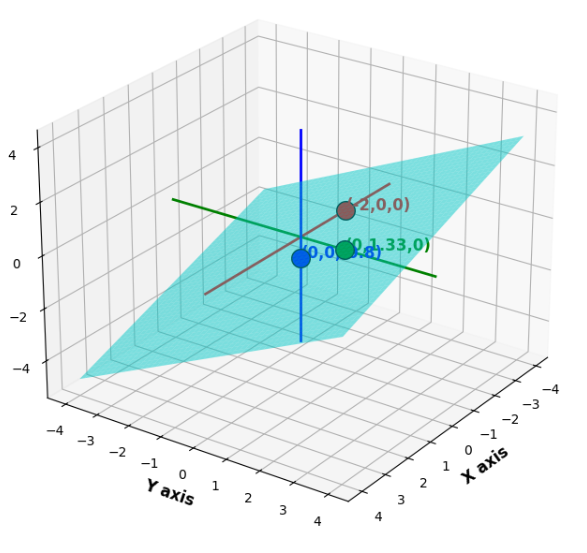
\includegraphics[width=0.5\columnwidth]{figs/graph.png}
\caption*{plane $2\text{x} - 3\text{y} + 5\text{z} + 4 = 0$ with intercepts}
\label{fig:graph.png}
\end{figure}  
\end{frame}
\end{document}